\documentclass[a4paper,11pt]{article}
\usepackage[utf8]{inputenc}
\usepackage[T1]{fontenc}
\usepackage[catalan]{babel}
\usepackage{amsmath}
\usepackage{amssymb}
\usepackage{amsfonts}
\usepackage{graphicx}
\usepackage{subcaption}
\usepackage{float}
\usepackage{fancyhdr}
\usepackage{geometry}

\geometry{
  left=25mm,
  right=25mm,
  top=30mm,
  bottom=30mm,
}

\setlength{\headheight}{13.6pt}
\pagestyle{fancy}
\fancyhf{}
\lhead{Entrega 2. Zeros de funcions.}
\rhead{Laia Lluís Blanch, Carlo Sala Gancho}
\cfoot{\thepage}

\begin{document}
\graphicspath{ {./imatges/} }
\section*{Problema 1}
\subsection*{(a)}
A partir de dos tipus de nodes, els equiespaciats i els de Chebyshev, tal com es proposa a la pràctica, calculem els dos polinomis interpoladors per la funció $f(x) = \frac{1}{1 + 25x^2}$ i en dibuixem les gràfiques amb el programa \textit{gnuplot} usant 181 punts definits com $x_k = -0,989 + 0,011k$, amb $k = 0, \ldots, 180$. Això ho fem pels casos de $n = 4,8,16,32$ nodes. Les gràfiques obtingudes són les següents:
  \begin{figure}[H]
  \begin{subfigure}{0.49\textwidth}
    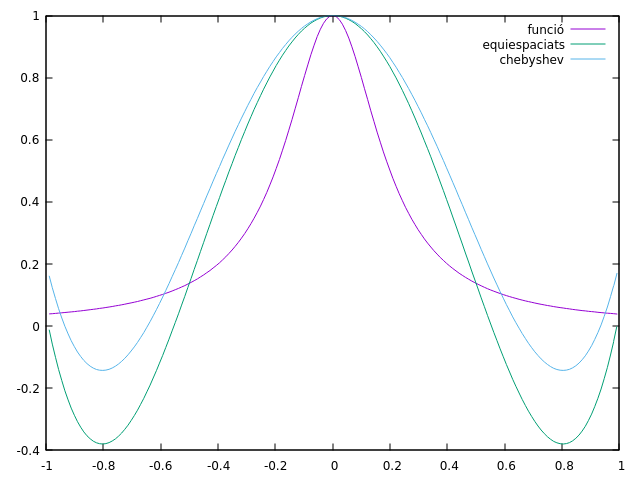
\includegraphics[width = 0.9 \linewidth]{imatges/plot4.png}
  \centering
  \caption*{$n = 4$}
  \end{subfigure}
  \begin{subfigure}{0.49\textwidth}
    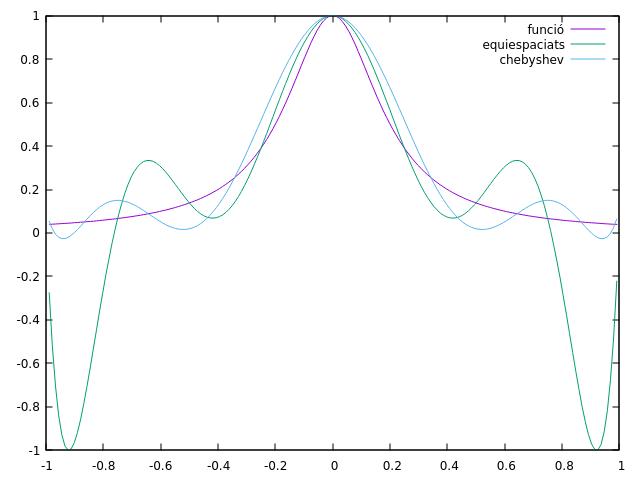
\includegraphics[width = 0.9 \linewidth]{imatges/plot8.png}
  \centering
  \caption*{$n = 8$}
  \end{subfigure}
  \end{figure}
  \begin{figure}[H]
  \begin{subfigure}{0.49\textwidth}
    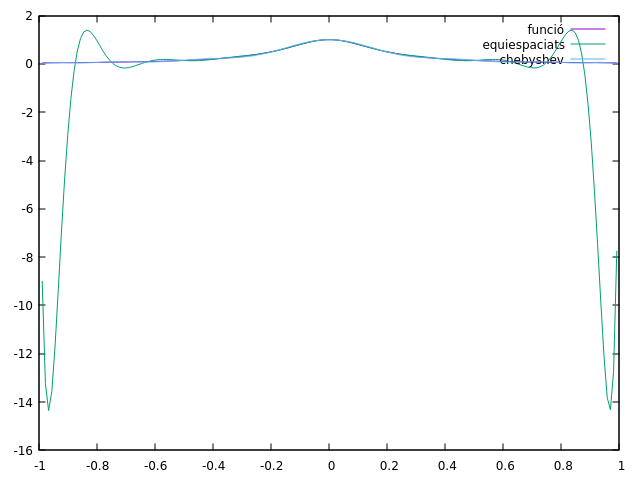
\includegraphics[width = 0.9 \linewidth]{imatges/plot16.png}
  \centering
  \caption*{$n = 16$}
  \end{subfigure}
  \begin{subfigure}{0.49\textwidth}
    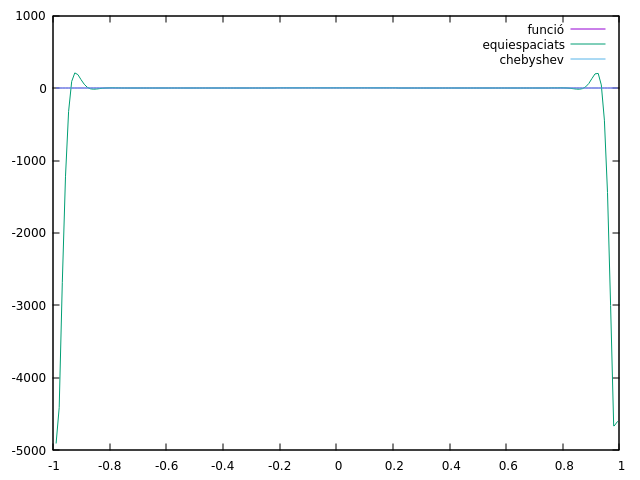
\includegraphics[width = 0.9 \linewidth]{imatges/plot32.png}
  \centering
  \caption*{$n = 32$}
  \end{subfigure}
  \end{figure}
  \begin{figure}[H]
  \begin{subfigure}{0.49\textwidth}
    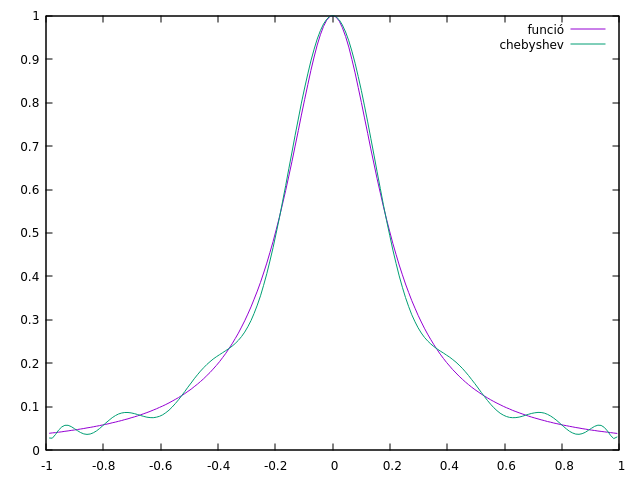
\includegraphics[width = 0.9 \linewidth]{imatges/plot16-noeq.png}
  \centering
  \caption*{$n = 16$ (sense equiespaciats)}
  \end{subfigure}
  \begin{subfigure}{0.49\textwidth}
    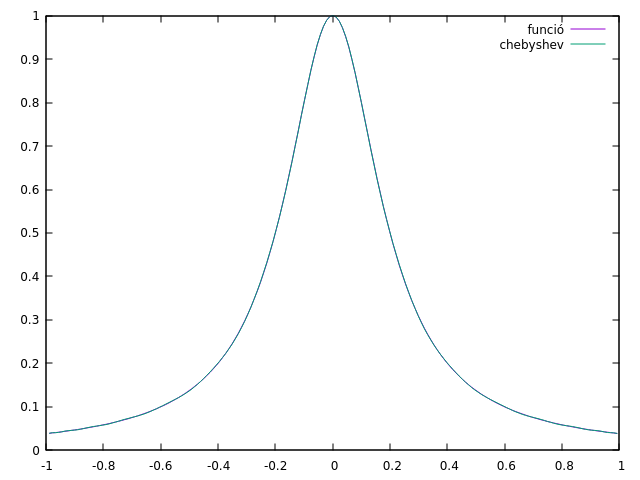
\includegraphics[width = 0.9 \linewidth]{imatges/plot32-noeq.png}
  \centering
  \caption*{$n = 32$ (sense equiespaciats)}
  \end{subfigure}
  \end{figure}
  Vegem que conforme anem augmentant el nombre de nodes (en el cas de Chebyshev) el polinomi interpolador cada vegada aproxima millor a la funció original. Per contra, quan fem servir els nodes equiespaciats i n'augmentem el nombre, cada vegada es comet més error i el polinomi interpolador aproxima pitjor a la funció original.\\
  Inferim, per tant, que agafar un nombre més gran de nodes no implica necessàriament millorar el polinomi interpolador i, a més, observem clarament que els nodes de Chebyshev fan una molt millor feina a l'hora de crear un polinomi interpolador per una funció.
\subsection*{(b)}
  Observem en les següents taules els diferents errors màxims comesos per cada un dels tipus de nodes i cada valor de $n$:
  \begin{table}[H]
  \begin{center}
    \begin{tabular}{|c|c|c|c|c|}
      \hline 
      $n$ & $4$ & $8$ & $16$ & $32$\\
      \hline
      $\left| f(x_k) - p(x_k) \right|$
      & 
      $0.438333$
      & 
      $1.044314$
      &
      $14.393851$
      &
      $4905.447137$
      \\
      \hline
    \end{tabular}
    \caption{Error màxim amb nodes equiespaiats}
  \end{center}
  \end{table}
  \begin{table}[H]
  \begin{center}
    \begin{tabular}{|c|c|c|c|c|}
      \hline 
      $n$ & $4$ & $8$ & $16$ & $32$\\
      \hline 
      $\left| f(x_k) - p(x_k) \right|$
      & 
      $0.401891$
      & 
      $0.170717$
      &
      $0.032538$
      &
      $0.001394$
      \\
      \hline
    \end{tabular}
    \caption{Error màxim amb nodes de Chebyshev}
  \end{center}
  \end{table}
  Observem que, tal com havíem previst a l'apartat (a), conforme anem augmentant el nombre de nodes de Chebyshev l'error cada vegada es fa més petit i el polinomi aproxima la funció d'una forma molt més acurada. De la mateixa manera, observem que els nodes equiespaciats cada vegada tenen un error més gran conforme augmentem el nombre de nodes, fins a arribar a un error dramàtic de gairebé 5000 per una funció que està acotada per $0$ i $1$. Per tant, el càlcul de l'error reforça la idea i conclusió que havíem tret de l'apartat (a).\\
  Per tant, els nodes de Chebyshev sempre seran una millor tria per davant dels nodes equiespaciats per poder crear un polinomi interpolador que aproximi de forma precisa una funció.
  \clearpage
\section*{Problema 2}
  En aquest problema se'ns planteja un mètode interessant a l'hora de resoldre arrels de certes equacions que, de sortida, semblen molt difícils de trobar. Per exemple, si intentéssim trobar l'arrel proposada a la pràctica de la funció $J_0(x)$ se'ns faria molt difícil, ja que només per derivar-la ja tindríem molta feina. Llavors, usant la interpolació inversa aconseguim simplificar i agilitzar el càlcul de $x^*$, entenent que $x^*$ és el valor que fa que $J_0(x^*) = 0$.\\
  Seguint amb aquesta idea, hem calculat el polinomi interpolador de Lagrange (usant les diferències dividides de Newton) de $J_0^{-1}(x)$, considerant els nodes els valors de $J_0(x)$ i les seves imatges els valors de $x$. Obtenim els següents resultats per cada un dels casos proposats a l'enunciat:
  \begin{table}[H]
  \begin{center}
    \begin{tabular}{|c|c|c|c|}
      \hline
      Grau & $1$ & $3$ & $5$ \\
      \hline
      Positius & $2.404729$ & $2.404823$ & $2.404825$ \\
      \hline
      Negatius & $2.400077$ & $2.404149$ & $2.404217$ \\
      \hline
      Simètrics & $2.404928$ & $2.404824$ & $2.404826$ \\
      \hline
    \end{tabular}
    \caption{Arrel de $J_0(x)$}
  \end{center}
  \end{table}
  Tenint en compte que la funció és estrictament monòtona i derivable, és a dir, que és suau, n'inferim que els millors resultats els obtenim de la interpolació de nodes positius i simètrics, ja que el node més proper a l'arrel de la funció és $J_0(2.4) = 0.002507683297244$, que és un valor positiu. En aquest cas, gràcies que la funció és monòntona, entenem també que, quants més nodes tinguem i més propers siguin a l'arrel, amb més precisió serem capaços de calcular l'arrel de la funció. En conclusió, la millor de les eleccions de valors a interpolar són els valors simètrics respecte l'arrel de la funció, ja que agafa valors propers a banda i banda de l'arrel.
\end{document}
